% Send to Mandar,Jayesh,Arnab,Deepak and perhaps Rahee, PEB, AAO, Michael Richards, John W, Jaydeep K, and Grace Gu, GR Gogate, Chaitanya Bapat, Shekhar Divekar, Hrishikesh, Shilpa, maybe Prem Andrade, Aaron Ashwin
\documentclass[12pt]{article}
\newcommand{\beq}{\begin{equation}}
\newcommand{\eeq}{\end{equation}}
\newcommand{\ber}{\begin{eqnarray}}
\newcommand{\eer}{\end{eqnarray}}
\newcommand{\nn}{\nonumber}
\newcommand{\dd}[2]{\frac{d}{d{#2}}{(#1)} }
\newcommand{\pdd}[2]{\frac{\partial}{\partial{#2}}{(#1)} }
\newcommand{\nhgscalefactor}{0.22}
\newcommand{\nhgfigheight}{3.8cm}
\usepackage{amsmath}
\usepackage{amsfonts}
\usepackage{cite}
\usepackage{url}
\usepackage{graphicx}
%\usepackage{caption}
\usepackage{subcaption}
%\usepackage{subfig}
\usepackage{multirow}
\usepackage{draftwatermark}
% usually hyperref has to be the last package imported
\usepackage{hyperref}
\SetWatermarkText{Draft}
\SetWatermarkScale{5}
%
\begin{document}
% bib
\title{Elasticity imaging using a Convolutional Neural Network}
\author{Nachiket Gokhale\footnote{The author is very grateful to Paul Barbone for patiently answering many questions about finite elements. Conversations with Arnab Majumdar, Michael Richards and Mandar Kulkarni are gratefully acknowledged and appreciated.}\\gokhalen@gmail.com}
\date{\today}
\maketitle
\abstract{We explore the application of a Convolutional Neural Network (CNN) using labeled data (supervised learning) to image the shear modulus field of an almost incompressible elastic medium in plane strain using displacement or strain field data. This problem is important in medicine because the shear modulus of suspicious and potentially cancerous growths in soft tissue is elevated by about an order of magnitude as compared to the background of normal tissue. Therefore, imaging the stiffness leads to high-contrast medical images. Our prediction problem is as follows: \textit{Given displacement or strain fields, predict the shear modulus field}. Our CNN is trained using 2400 training examples consist of displacement or strain fields and a corresponding shear modulus field. We present encouraging results which warrant further research and show the promise of this methodology.}
\section{Introduction}
The shear modulus of palpable nodules (which can be thought of as abnormal and potentially cancerous growths in soft tissue) is approximately an order of magnitude higher than the stiffness of the background of normal glandular tissue \cite{paper:sarv1998}. See also Figure (\ref{fig:shearmod}). It follows then, that imaging the shear modulus of soft tissue results in a high-contrast imaging method because suspicious growths will stand out clearly against the background of normal tissue. Elasticity Imaging is a broad term that refers to methods which image the shear modulus (or other elastic properties) of soft tissue in various ways. See \cite{paper:gao1996,paper:parker2010,book:alamgarra2019,bookchap:oberaibarbone2019} for a comprehensive reviews of the field.
%
\begin{figure}
   \centering
    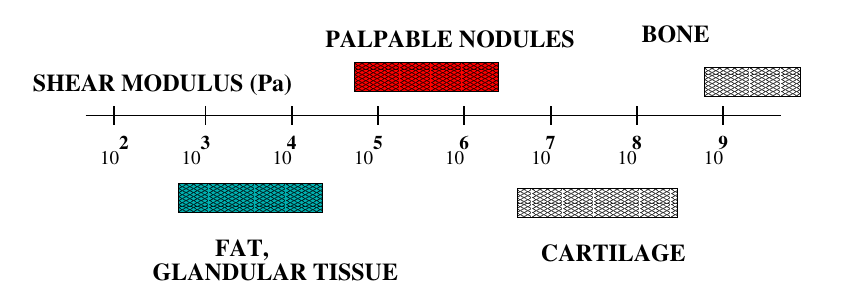
\includegraphics[totalheight=3cm]{Figures/shearmod.png}
  \caption{\label{fig:shearmod} Shear moduli of different types of soft tissue. Adapted from Figure 1 in \cite{paper:sarv1998}.}
\end{figure}
%
\begin{figure}
   \centering
    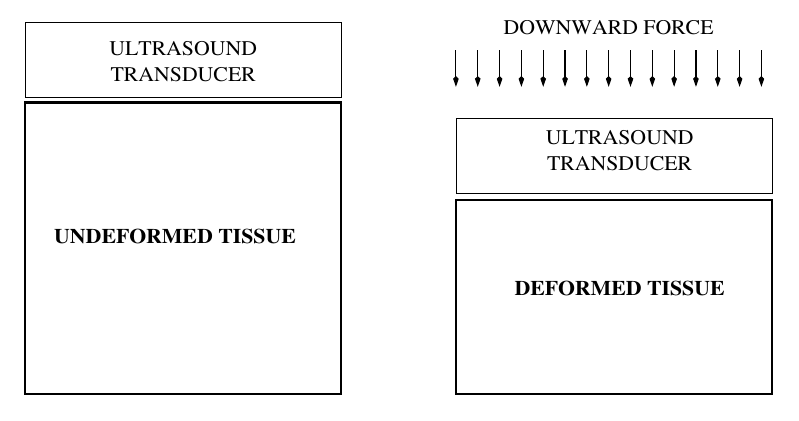
\includegraphics[totalheight=5cm]{Figures/prepostimage.png}
  \caption{\label{fig:prepostimage} Schematic figure showing medical image acquisition when soft tissue is being deformed using ultrasound imaging. The image taken on the left is referred to as the \textit{pre-deformation} image and the image on the right is the \textit{post-deformation image}.}
\end{figure}
%
\subsection{Steps involved in elasticity imaging}
Elasticity Imaging typically consists of  the steps of image acquisition, image registration, and inverse problem solution. These steps are discussed in the following sections.
\subsubsection{Image acquisition} Images of soft tissue undergoing deformation are acquired using various imaging modalities such as ultrasound or magnetic resonance imaging. While time dependent images can be acquired, we shall consider here only two images: a \textit{pre-deformation image} acquired before force is applied and a \textit{post-deformation image} acquired after force is applied. This process is shown in Figure (\ref{fig:prepostimage}) for ultrasound imaging. Also see Figure 2 in \cite{paper:konofagou2004}.
\subsubsection{Image registration} The goal in this step is to find a map between the pre-deformation image and the post-deformation image. For every point in the pre-deformation image we aim to find its location in the post-deformation image. This gives us the \textit{displacement field} between the two images. This displacement field is often referred to as the \textit{measured displacement field}. See \cite{paper:richards2009,paper:gokhale2004,paper:pellot-barakat2004} for minimization based approaches for computing the displacement field. See \cite{paper:ophir1991,paper:ophir1996,paper:alam1998} and references therein for cross-correlation based approaches.
\subsubsection{Inverse problem solution:} The goal in this step is to infer the spatial distribution of the shear modulus from the displacement field. This is called an \textit{inverse problem} because the typical boundary value problem in linear elasticity (referred to as the \textit{forward problem}) is to determine the displacement field given the shear-modulus field. The approaches for inverse problem solution can be divided into two categories: direct and iterative.
\subsubsection{Direct approach} Direct approaches involve solving a single partial differential equation (pde) to obtain the distribution of shear modulus directly: see \cite{paper:raghavan1994,paper:barboneadjwt,paper:albocher}. The coefficients of this pde depend on the measured displacement field. Such approaches are fast and work well when the measured strain field is completely known and has low noise.
\subsubsection{Iterative approach} Iterative approaches \cite{paper:oberai2003,paper:gokhale2008,paper:kalle1996,paper:doyley,paper:goenezen2011} involve guessing a distribution for the shear modulus, solving a linear elasticity forward problem to obtain the predicted displacements, comparing the predicted displacements to the measured displacements and updating the guessed shear modulus distribution using a suitable optimization procedure such as a modified Newton Raphson scheme as in \cite{paper:doyley} or the BFGS scheme as in \cite{paper:gokhale2008,paper:goenezen2011}. Such approaches are typically slower than direct methods, since the require the solution of $\approx$ 25-100 forward problems, but have the ability to handle incomplete data and complex material models.
\subsection{Solving the inverse problem with CNNs}
We believe that solving the inverse problem with CNNs can combine the best characteristics of the direct and iterative approaches. The CNN based approach can yield a quick answer, can accomodate complex constitutive relations, can work with incomplete data (e.g. only a single component of a displacement field) and can work with noisy data.
\section{Neural networks and problem setup}
In recent years, neural networks have been applied to various applications such as image classificaton \cite{paper:hinton2017}, hand written digit recognition \cite{paper:kulkarni2018}, solving differential equations and symbolic integration \cite{misc:lample2019}, solving complex partial differential equations such as the Navier-Stokes equation \cite{misc:anandkumar2020}, self-driving cars \cite{misc:agnihotri2019,misc:nvidiaselfdriving2016}, chaos \cite{paper:pathak2018}, natural language processing \cite{misc:googlenlp} and face recognition \cite{conf:taigman2014}. Several effective Machine Learning frameworks such as Google's TensorFlow \cite{misc:tensorflow}, Facebook's PyTorch \cite{incollect:pytorch}, Scikit-Learn \cite{paper:scikit-learn} are freely available. See \cite{misc:compdeep} for a complete list. The interested reader is referred to \cite{book:aggarwal,book:goodfellow,book:chollet,misc:cs231n,misc:andrewng,misc:udemy} for further information about neural networks.
\subsection{Neural networks and elasticity imaging}
Given the success achieved by neural networks on the wide variety of applications cited, it is natural to explore the application of neural networks to the inverse problem of elasticity imaging and several recent efforts \cite{paper:pateloberai2019,misc:gu2020,paper:hoeriginsana2016} have done so. In \cite{paper:pateloberai2019}, the authors use a convolutional neural network to classify specimens into elastically heterogeneous or elastically nonlinear. In \cite{paper:hoeriginsana2016}, the authors use a neural network to estimate strains and stress and then calculate elastic parameters. In \cite{misc:gu2020}, the authors use a neural network which predicts elasticity distributions using residual force maps to update the weights of the neural network. \\In contrast, in this work we compute the shear modulus field from the displacement or strain field using a CNN. There are no physical constraints involved in our work. It is purely a mapping problem from the space of displacement or strain fields to the space of the shear modulus fields. We supply our CNN with labeled data which consists of strain or displacement fields and shear modulus fields. Based on this data, the CNN learns weights for its filters and other parameters. Using this learned information the CNN is able to predict a shear modulus field from the input data of strain or displacement fields.
%
\subsection{\label{sect:cnnarch} CNN architecture used in this work}
The typical architecture of the CNN we use in this work is shown in Figure (\ref{fig:typical_cnn}) and its parameters are given in Table (\ref{tab:cnnparams}). This CNN was implemented in TensorFlow \cite{misc:tensorflow}. The first dimension '?' represents the number of examples to be processed for training, validation or evaluation. Thus, the first training example is a three dimensional array and can be accessed using the indices $[0,:,:,:]$ (using Numpy notation) and similarly for the others. The second and third dimensions represent the number of nodes in the $y$ and $x$ direction respectively. The last dimension represents the number of channels in the image. In image-processing the number of channels is typically $3$, one channel each for the three colors red, green and blue (RGB). In our case, the number of channels is the number of independent fields in our problem. If we use three independent components of the strain field $\epsilon_{xx},\epsilon_{yy},\epsilon_{xy}$ then the number of channels is $3$. If we use only a single component of the strain field, say $\epsilon_{xx}$ only, then the number of channels is $1$. The \textit{loss function} is \textit{mean squared error} and the optimizer is \textit{Adam}. No regularization is used.  Each CNN has approximately $3.35$ million trainable parameters.
\begin{table}
  \centering
 \begin{tabular}{|c|c|}
   \hline
   CNN Layer & Specifications \\
   \hline
   conv2d    & $32$ filters, kernel size $3$, activation is \textit{relu}, no regularization\\
   \hline
   max\_pooling2d: & pool size $2$, strides $2$\\
   \hline
   conv2d\_1 & $64$ filters, kernel size $3$, activation is \textit{relu}, no regularization\\
   \hline
   max\_pooling2d\_1: & pool size $2$, strides $2$\\
   \hline
   flatten & -\\
   \hline
   dense   & $128$ units, activation \textit{relu}, no regularization\\
   \hline
   dense\_1 & $nnodex*nnodey$ units, activation \textit{softplus}, no regularization\\
   \hline
 \end{tabular}
 \caption{\label{tab:cnnparams} CNN parameters for the network in Figure (\ref{fig:typical_cnn}).}
\end{table}
%
\begin{figure} 
   \centering
    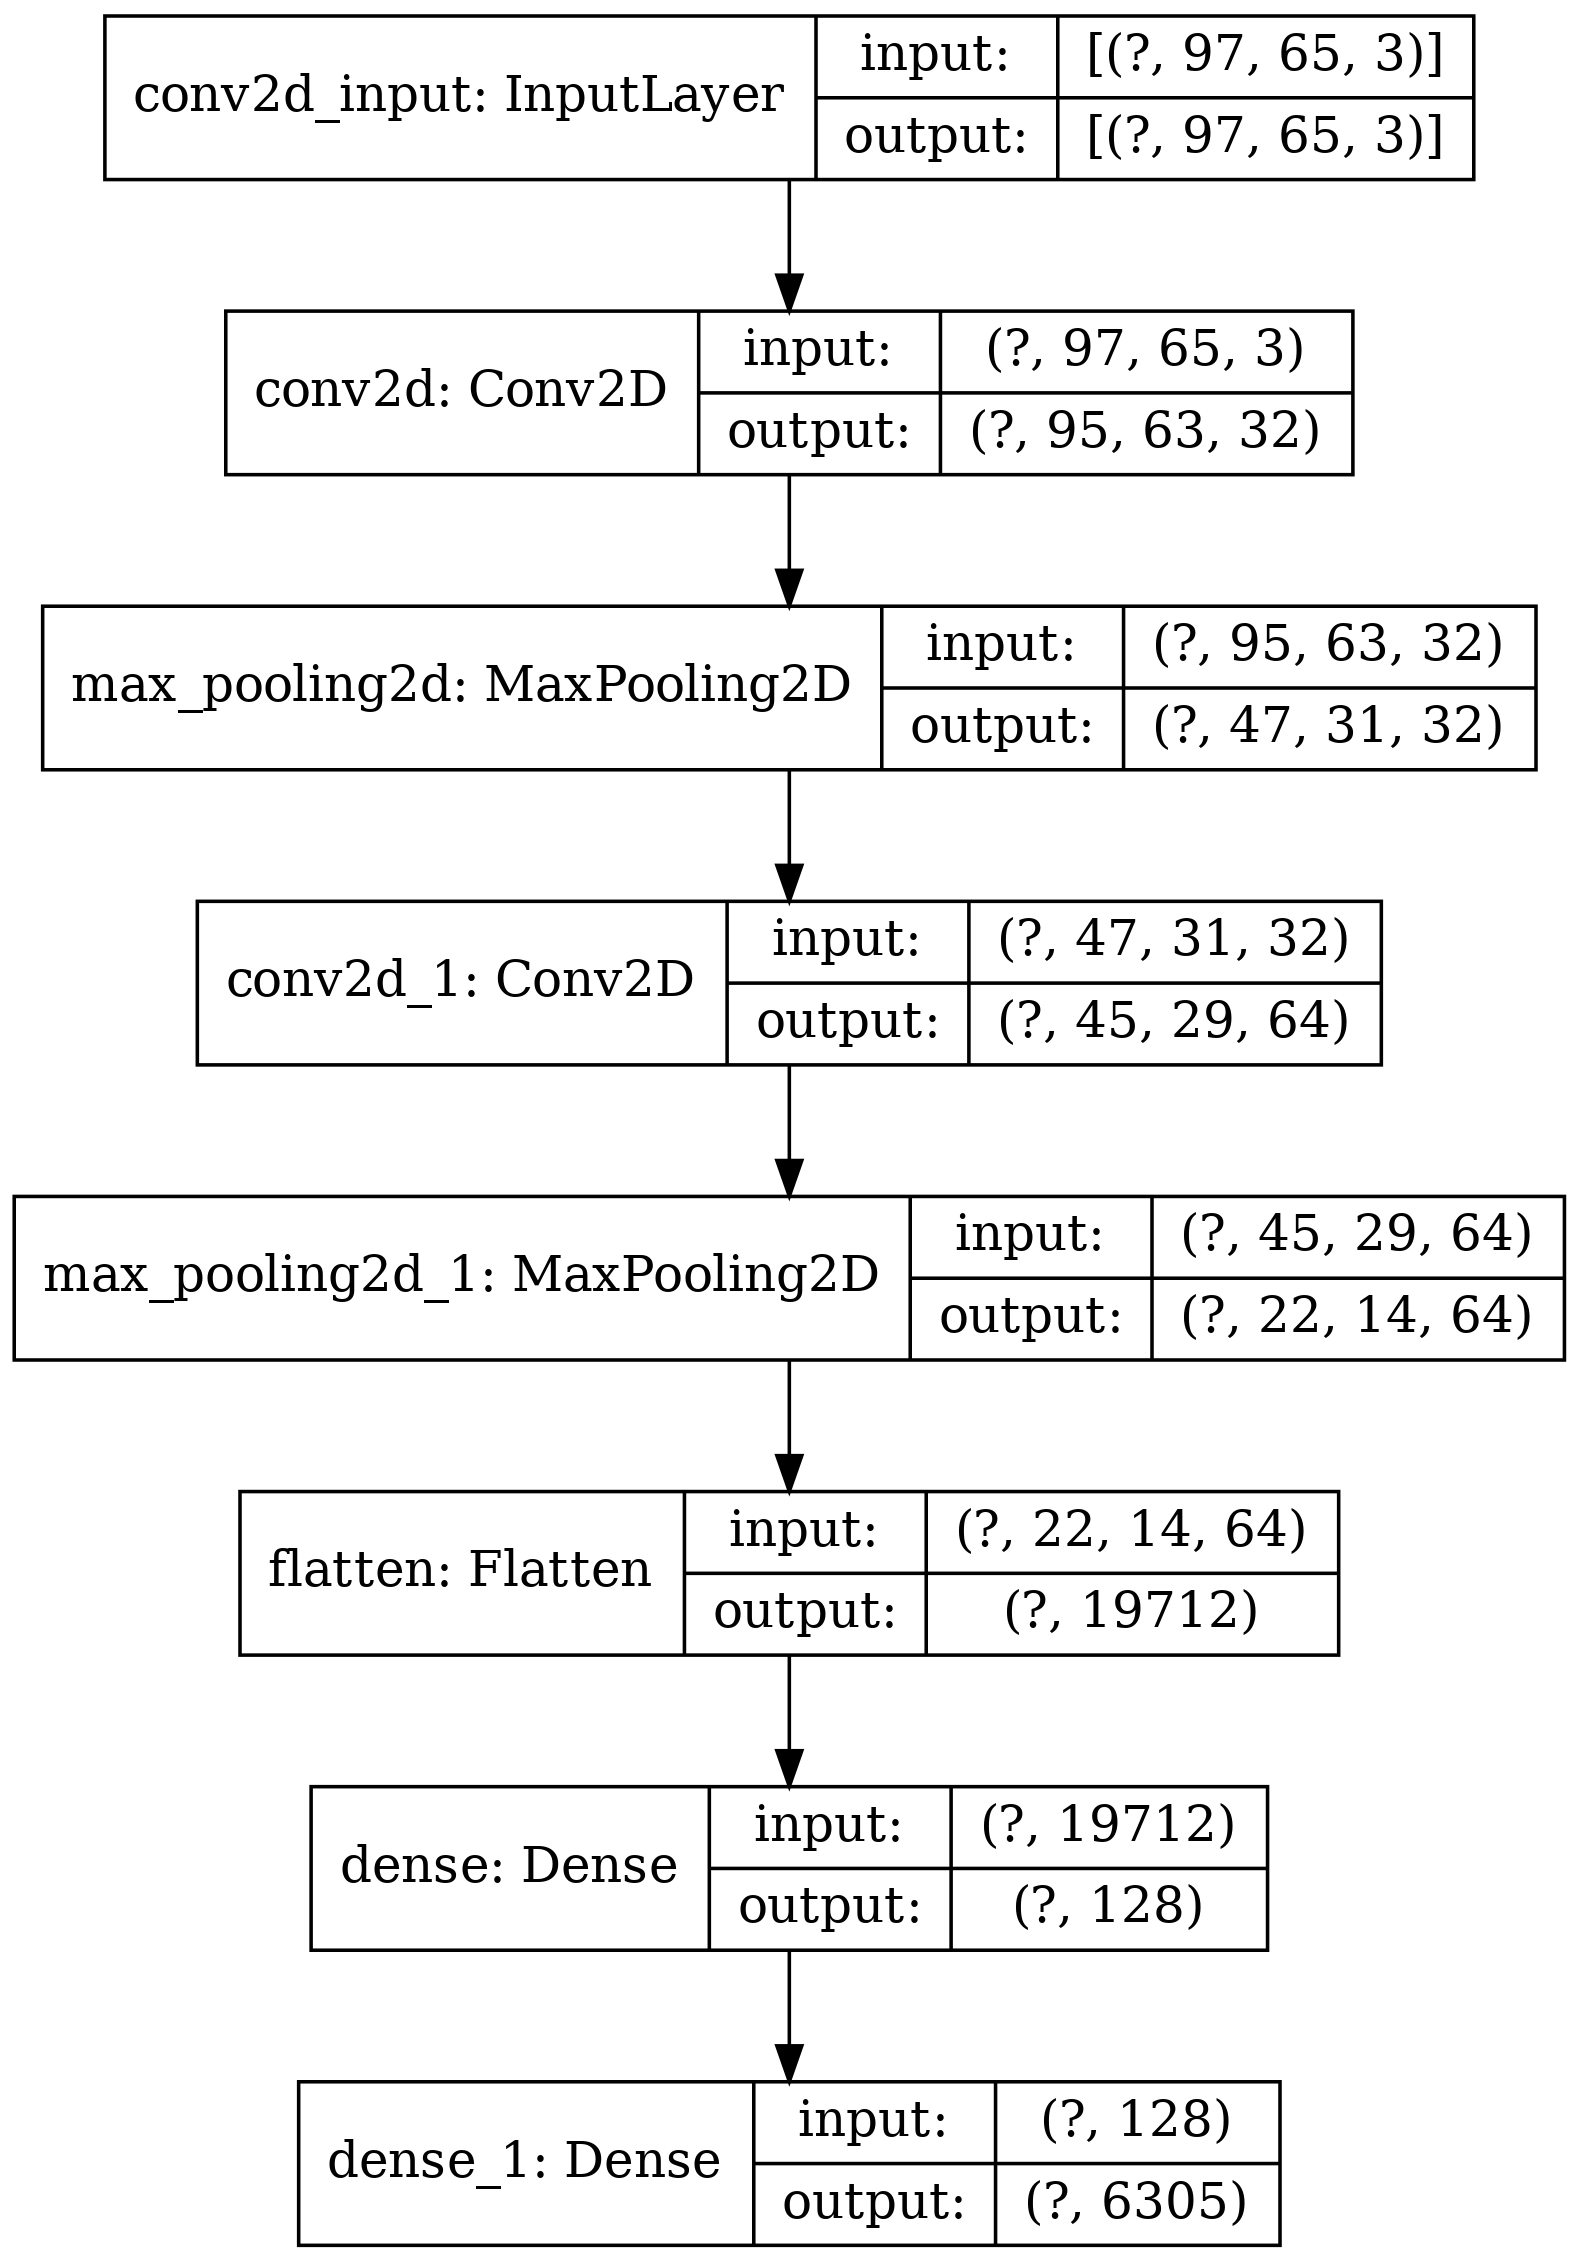
\includegraphics[totalheight=9cm]{Figures/typical_cnn.png}
    \caption{\label{fig:typical_cnn}Typical CNN architecture used in this work. This architecure is essentially the same the one used in the Deep Learning example in \cite{misc:udemy}.}
\end{figure}
%
%
\subsection{\label{sect:probsetup}Problem setup}
The displacement or strain field data required for the CNN is generated using a linear finite element solver named FyPy (\textbf{Fy}nite Elements in \textbf{Py}thon) \cite{misc:fypy}. The problem geometry is shown in Figure (\ref{fig:bc}). The length (in the $x$ direction) is $1.0$ unit. The breadth (in the $y$ direction) is 1.5 units. The background shear modulus is $1.0$ unit. The Poisson's ratio is a constant and is set to $0.49$. There is exactly one inclusion in the domain and its shear modulus is a constant and is a random number ranging from $2.0$ to $5.0$. There are no homogeneous examples. The radius of the inclusion is a random number randing from $0.05$ to $0.15$. $4000$ displacement and strain images are generated and are split into $2400$ training examples, $800$ validation examples and $800$ test examples. When noisy data is used we add noise in the strain or displacement data such that the signal to noise ratio (SNR) is 40dB using equation (\ref{eqn:snr}). The data is made noisy by element wise multiplication of the strain or displacement data with a matrix containing random numbers in the interval $(1-\epsilon,1+\epsilon)$. $\epsilon$ is chosen appropriately to yield $\approx$ 40dB noise
\begin{equation}
  \label{eqn:snr}
  SNR_{dB} = 20\log_{10}\Big(\frac{\|signal\|}{\|noise\|}\Big)
\end{equation}
% Noise details
%
\begin{figure} 
   \centering
    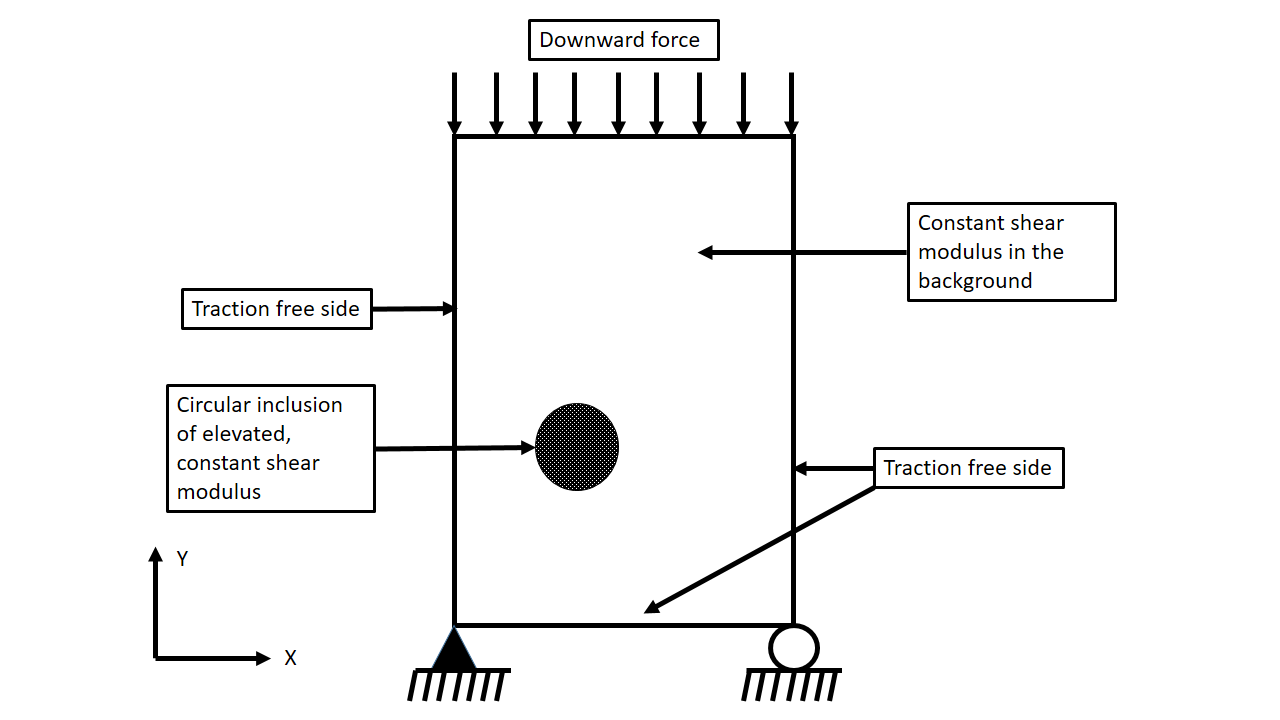
\includegraphics[totalheight=9cm]{Figures/bc.png}
  \caption{\label{fig:bc}Boundary conditions and material properties used in this work. }
\end{figure}
%
\section{Imaging one inclusion}
\subsection{Case 1: Using $\epsilon_{xx}$ and $\epsilon_{yy}$}
% loss and val_loss Curves
\subsection{Case 2: Using $\epsilon_{yy}$ only}
% loss and val_loss Curves
\subsection{Case 3: Using $u_x$ and $u_y$}
% loss and val_loss Curves
\subsection{Case 4: Using $u_y$ only}
% loss and val_loss Curves
\pagebreak
\begin{figure}
  \centering
  %
  \begin{subfigure}[b]{\nhgscalefactor\linewidth}
    \includegraphics[totalheight=\nhgfigheight]{Figures/strain/ex1/mucomp00.png}
    \caption{True}
  \end{subfigure}
  %
   \begin{subfigure}[b]{\nhgscalefactor\linewidth}
    \includegraphics[totalheight=\nhgfigheight]{Figures/strain/ex1/mucomp00.png}
    \caption{$\epsilon_{xx}+\epsilon_{yy}$}
   \end{subfigure}
   %
   \begin{subfigure}[b]{\nhgscalefactor\linewidth}
    \includegraphics[totalheight=\nhgfigheight]{Figures/strain/ex1/mucomp00.png}
    \caption{(b) + noise}
   \end{subfigure}
   %
   \begin{subfigure}[b]{\nhgscalefactor\linewidth}
    \includegraphics[totalheight=\nhgfigheight]{Figures/strain/ex1/mucomp00.png}
    \caption{$\epsilon_{yy}$}
   \end{subfigure}
   %
   \begin{subfigure}[b]{\nhgscalefactor\linewidth}
     \includegraphics[totalheight=\nhgfigheight]{Figures/strain/ex1/mucomp00.png}
     \caption{$\epsilon_{yy}$+noise}
   \end{subfigure}
   \begin{subfigure}[b]{\nhgscalefactor\linewidth}
     \includegraphics[totalheight=\nhgfigheight]{Figures/strain/ex1/mucomp00.png}
     \caption{$u_x+u_y$}
   \end{subfigure}
   %
   \begin{subfigure}[b]{\nhgscalefactor\linewidth}
     \includegraphics[totalheight=\nhgfigheight]{Figures/strain/ex1/mucomp00.png}
     \caption{$u_y$}
   \end{subfigure}
   %
   \begin{subfigure}[b]{\nhgscalefactor\linewidth}
     \includegraphics[totalheight=\nhgfigheight]{Figures/strain/ex1/mucomp00.png}
     \caption{$u_y$+noise}
   \end{subfigure}
  \caption{\label{app:eyy:curves} Optmization history during the training phase for binary classification using $\epsilon_{yy}$ only.}
\end{figure}
\clearpage
\newpage
%
\section{Imaging multiple inclusions}
%
%
\section{Movie test}
\href{run:movies/movie.mp4}{\includegraphics[height=0.7\textwidth]{movies/mucomp00.png}}
\section{Conclusions and future work}
% Custom activation function
% https://stackoverflow.com/questions/43915482/how-do-you-create-a-custom-activation-function-with-keras
\begin{enumerate}
\item{Checkpoint and save best weights instead of just running for $512$ epochs. https://stackoverflow.com/questions/42666046/loading-a-trained-keras-model-and-continue-training}
\item{Use prior knowledge to improve performance. e.g. if we know that radius can lie between 1 pixel and 3 pixels, perhaps we can use that information to improve performance. Similarly if we know that stiffness can lie between specifed ranges, then use that knowledge to constrain NN output}
\item{Better results are obtained for larger inclusion with larger contrast}
\item{Larger datasets: 100,000 or so datasets}
\item{Better NN architectures. Shallower or deeper.}
\item{Mapping medical images to shear modulus directly skipping registration.}
\item{Training multiple NNs on the same data set using different initializations for the weights. One can then average the prediction or average the weights.}
\item{Handling noise: augmenting dataset by adding noise to displacement/strain fields}
\item{Stiffness is always underpredicted. Smaller inclusions are not handled well. Larger inclusions are handled better. Maybe having material properties and displacements on the same mesh leads to unconverged displacements for smaller inclusions. These unconverged displacements will not have enough features/information to be able to predict stiffness fields from them.}
\item{Actual material properties and breast/organ geometry}
\item{Multiple displacement fields: In \cite{paper:barbonegokhale,paper:barbonebamber} the authors show that a single strain or displacement field is not sufficent to predict the shear modulus field uniquely and multiple displacement fields are required for unique prediction of the shear modulus field. The use of multiple displacement fields can be considered within our current framework. This would involve increasing the number of channels in a dataset. See Section (\ref{sect:cnnarch}) for more information on channels.} 
\item{Software and performance issues: The finite element solver and associated scripts for generating the data were written in Python 3.8. Python is slow and much better performance could be obtained by writing the solver in C/C++/Fortran or Julia or using open source solvers like FEniCS \cite{paper:fenics} or deal.II \cite{misc:deal.ii}. Each FE input file is 3.3MB and output file is 1.1MB and total dataset size $\approx$  20GB. There was no effort made to minimize the size of input and output files. Simple text based JSON files were used. If one wants increase the number of training examples by a factor of thousand 17TB of data would be required. Optimized data structures and hardware supporting fast disk access (SSDs) will be necessary for scaling to a large data sets. The use of GPU clusters to process large amounts of data may also need to be considered. }
\end{enumerate}
\bibliography{eibib}{}
\bibliographystyle{plain}
\end{document}


% Document ends here

\appendix


\section{\label{sect:binary}Binary classification}
In this section, we consider the problem of identifying whether or not there is an inclusion in an elastic domain from given one component of strain or displacement fields. The CNN used in this section is essentially the same the one described in Section (\ref{sect:cnnarch}) with the following changes. The dense output layer contains only $1$ node, its activation is \textit{sigmoid} and the loss function is \textit{binary cross entropy}. The geometry of the examples is as described in Section (\ref{sect:probsetup}) and Figure (\ref{fig:bc}). The training set consists of $1024$ examples out of which $200$ are homogenous with shear modulus of $1$ unit and the rest contain a single inclusion. The shear modulus of the single inclusion is a constant and is a random number between $2.0$ and $5.0$. The location of the inclusion is random and its radius is a random number between $0.05$ and $0.15$. The examples with the inclusion present are labeled '$1$' and the examples without an inclusion are labeled '$0$'. The validation and test data sets contain $204$ examples each out of which $40$ are homogeneous and the rest have an inclusion.
% loss and val_loss Curves
\subsection{Case 1: Using $\epsilon_{yy}$ with no noise}
The training history for this case is shown in Figure (\ref{app:eyy:curves}).
% figures for loss,val_loss,val_accuracy
\begin{figure}
  \centering
  %
  \begin{subfigure}[b]{0.45\linewidth}
    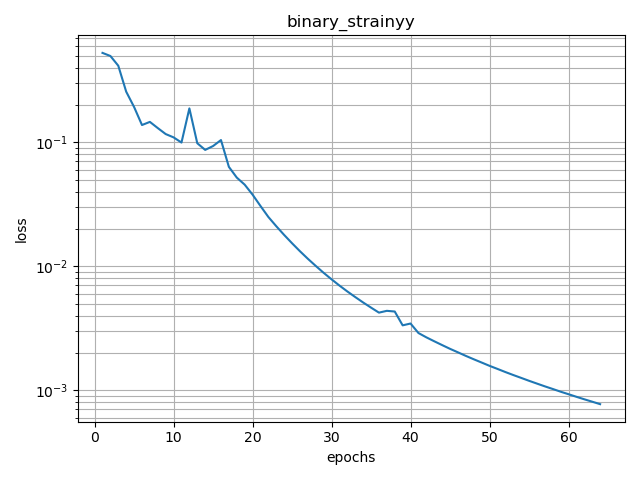
\includegraphics[totalheight=4cm]{Figures/Appendix/eyy/binary_strainyy_plot_loss.png}
    \caption{True}
  \end{subfigure}
  %
   \begin{subfigure}[b]{0.45\linewidth}
    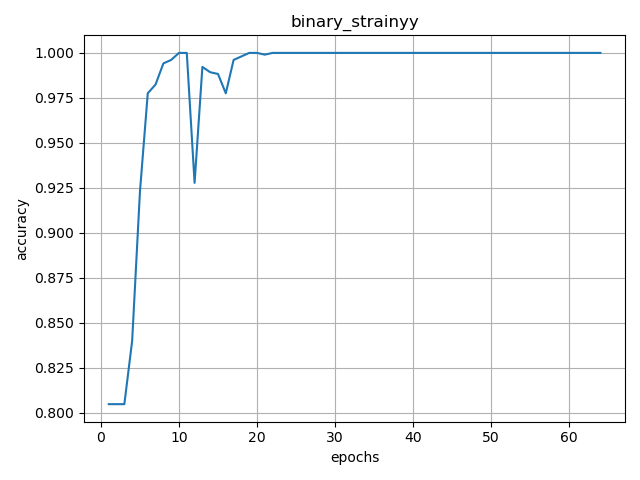
\includegraphics[totalheight=4cm]{Figures/Appendix/eyy/binary_strainyy_plot_accuracy.png}
    \caption{Training accuracy vs epochs}
   \end{subfigure}
   %
   \begin{subfigure}[b]{0.45\linewidth}
    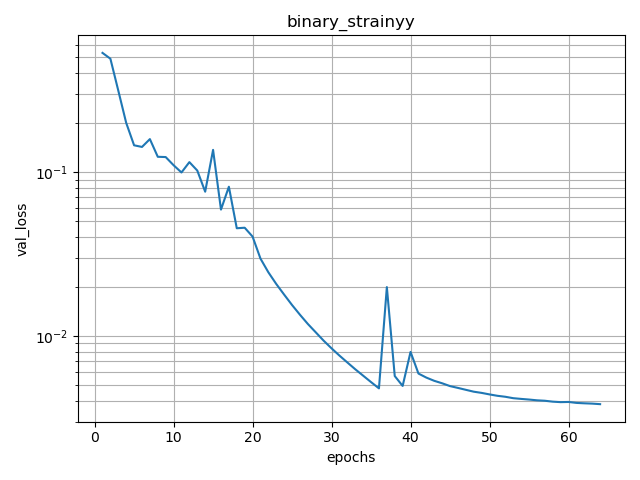
\includegraphics[totalheight=4cm]{Figures/Appendix/eyy/binary_strainyy_plot_val_loss.png}
    \caption{Validation loss function vs epochs}
   \end{subfigure}
   %
   \begin{subfigure}[b]{0.45\linewidth}
     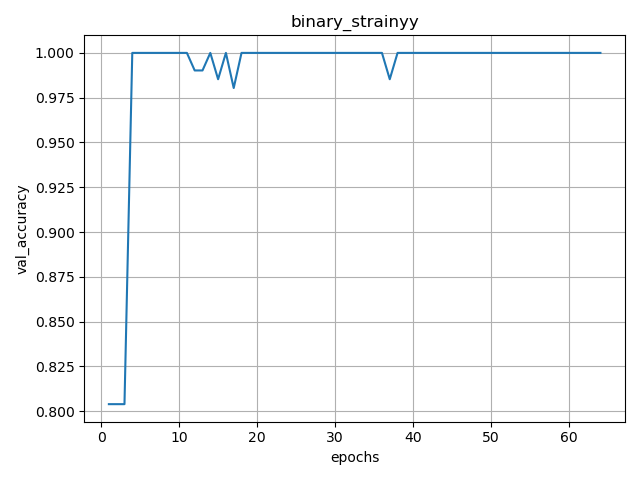
\includegraphics[totalheight=4cm]{Figures/Appendix/eyy/binary_strainyy_plot_val_accuracy.png}
     \caption{Validation accuracy vs epochs}
   \end{subfigure}
   %
  \caption{\label{app:eyy:curves} Optmization history during the training phase for binary classification using $\epsilon_{yy}$ only.}
 \end{figure}
% loss and val_loss Curves
\subsection{Case 2: Using $\epsilon_{yy}$ with noise}
\subsection{Case 3: Using $u_y$ with no noise}
% loss and val_loss Curves
\subsection{Case 4: Using $u_y$ with noise}
%

